\documentclass[11pt]{amsart}
%\documentclass[11pt,a4paper]{amsart}

% use up more of the page
\addtolength{\topmargin}{-5mm}
\addtolength{\textheight}{12mm}
\addtolength{\oddsidemargin}{-9mm}
\addtolength{\evensidemargin}{-9mm}
\addtolength{\textwidth}{20mm}

%\usepackage[latin1]{inputenc}
\usepackage{amsmath}
\usepackage{natbib}
\usepackage{fancyvrb}
\usepackage[final]{graphicx}

% hyperref should be the last package we load
\usepackage[pdftex,
                colorlinks=true,
                plainpages=false, % only if colorlinks=true
                linkcolor=blue,   % only if colorlinks=true
                citecolor=black,   % only if colorlinks=true
                urlcolor=magenta     % only if colorlinks=true
]{hyperref}


\newcommand{\RR}{\mathbb{R}}

\newcommand{\Hij}{H_{i,j}}
\newcommand{\Pij}{P_{i,j}}
\newcommand{\Wij}{W_{i,j}}
\newcommand{\Yij}{Y_{i,j}}

\newcommand{\bF}{\mathbf{F}}
\newcommand{\bQ}{\mathbf{Q}}
\newcommand{\bW}{\mathbf{W}}

\newcommand{\bn}{\mathbf{n}}
\newcommand{\bq}{\mathbf{q}}
\newcommand{\bs}{\mathbf{s}}
\newcommand{\bv}{\mathbf{v}}

\newcommand{\hpw}{\hat P}
\newcommand{\Cavit}{C_{avit}}
\newcommand{\Creep}{C_{reep}}



\title[PISM hydrology model]{A subglacial hydrology model \\for the Parallel Ice Sheet Model (PISM)}

\author[van Pelt and Bueler]{Ward van Pelt and Ed Bueler}


\begin{document}

\maketitle

\begin{quote}
\textbf{Abstract}:  \emph{The drainage model we propose for PISM is inspired by the hydrology models of \emph{\citet{FlowersClarke2002_theory}},  \emph{\cite{Schoofmeltsupply}}, \emph{\citet{PimentelFlowers2011}}, and \emph{\citet{Hewitt2011}}.  A nonlinear diffusion for water amount is at the core of the model.  It is a form of the porous medium equation because we suppose a relationship (closure) between the water pressure and the water amount.  There is an evolution equation for aquifer capacity which has physical opening and closure terms. We numerically approximate the equations by an implicit time-stepping scheme using a parallel Newton method.  We address verification of the numerical scheme, the degree to which the model scales to large ice sheets, and parameter identification using GPS data.}
\end{quote}

\thispagestyle{empty}
\medskip

\section{Introduction}

Our goal is to capture the major qualities of an evolving drainage system, without over-specifying a particular system morphology.  We want to limit the number of unknown parameters.  The qualities captured by our model are:
\renewcommand{\labelenumi}{\emph{(\roman{enumi})}\quad}
\begin{enumerate}
\item liquid water lives in a sheet-like system and is conserved,
\item water flows from high to low hydraulic potential,
\item the capacity of the drainage system, described by an aquifer thickness parameter, evolves according to physical opening and closing processes,
\item water pressure is a increasing function of the ratio of water amount over capacity, and finally
\item changes in the basal resistance field (yield stress), which determines the basal shear stress under the ice sheet, depends on the water pressure.
\end{enumerate}

Our model simplifies the \citet{FlowersClarke2002_theory} model by assuming constant hydraulic conductivity, but, like \citet{Hewitt2011} we add \emph{(iii)}.  By \emph{(iv)}, the pressure is an increasing function of the water amount for fixed capacity, and it is a decreasing function of capacity for fixed water amount.  The stability of our sheet-like model is justified, in part, by the bed protrusion argument of \citet{CreytsSchoof2009}.  Our model differs from those of \citet{CreytsSchoof2009} and \citet{Hewitt2011} because we give evolution equations for water thickness and capacity separately.

We will connect this hydrology model to ice dynamics in a flexible and generic manner that can be applied by PISM users to ice sheets and glaciers.


\section{Subglacial aquifer model}

\subsection*{Thin-sheet subglacial water layer with Darcy flux}
The evolution of the water thickness $W(t,x,y)$ is described by the mass conservation equation,
\begin{equation} \label{eq:conserve}
\frac{\partial W}{\partial t} + \nabla \cdot \bQ = \Phi \, ,
\end{equation}
where $\bQ$ is the water flux, with units $\text{m}^2\,\text{s}^{-1}$, and $\Phi$ is a source term.

We may write the water sources
\begin{equation} \label{eq:watersources}
  \Phi = \frac{1}{\rho_w} \left(m + S\right)
\end{equation}
where $\rho_w$ is the density of fresh liquid water, $m$ is the rate at which basal melting (refreeze) of ice adds (removes) water, and $S$ is the rate at which surface runoff or englacial drainage adds water.  Groundwater could also contribute to the aquifer \citep[e.g.][]{DeFooretal2011}, and this would be included in $\Phi$, but we do not attempt to model such a contribution here.  Note $m$ and $S$ have mass per area per time units ($\text{kg}\,\text{m}^{-2}\,\text{s}^{-1}$), while $\Phi$ has units $\text{m}\,\text{s}^{-1}$.

In this paper we assume that $\Phi=\Phi(t,x,y)$ is a known function, but in applications $m$ and $S$ are coupling terms to other components of PISM.  In particular, basal melt $m$ is a function of the conservation of energy model \citep{AschwandenBuelerKhroulevBlatter}, while surface drainage $S$ is related to ice geometry and surface mass/energy processes \citep[e.g.][]{vanPeltetal}.  We will return to the parameterization of melt in a later subsection.

The layer thickness $W$ here is only meaningful if it is regarded as an average over a horizontal scale of tens or hundreds of meters, or more.  The numerical schemes used to discretize this model have horizontal cell sizes of a hundred meters up to $10$ km.  Process models for the evolution of channels, the geometry of cavities, the transport of sediment, the penetration of ice into the mineral base, and many other details of aquifer morphology are, of necessity, beyond the scope of this article.

We use a Darcy flux in our sheet-like formulation, as follows.  We express the water flux $\bQ$ in terms of a hydraulic potential $\psi$ \citep{Clarke05, FlowersClarke2002_theory} with units of pressure (Pa):
\begin{equation}
\bQ = - \frac{K \, W}{\rho_w g} \nabla \psi
\label{eq:flux}
\end{equation}
Here, $\rho_w$ is the water density, $g$ the gravitational acceleration and $K$ the effective hydraulic conductivity.  The hydraulic conductivity $K$ combines with the capacity thickness variable (called ``$Y$'' and introduced in the next section) to determine the transmissivity of the system \citep{PimentelFlowersSchoof2010}, but we take $K$ to be a positive constant.  Water flows from high to low fluid potential, by the negative sign in \eqref{eq:flux}.

The hydraulic potential (head) $\psi$ combines the water pressure $P(t,x,y)$ and the bedrock elevation $z=b(x,y)$:
\begin{equation} \label{eq:potential}
\psi = P + \rho_w g\, b \, .
\end{equation}
Thus from equation \eqref{eq:flux}, flow depends on both horizontal gradients in the water pressure and on the bedrock slope.

\subsection*{Empirical law for water pressure}  Subglacial water pressure is always related in some manner to the downward normal stress from the ice, the overburden stress.  We choose a particular form for the overburden stress, the standard cryostatic choice \citep{Clarke05}.  Conceptually, we identify the normal stress with the ice pressure $p_i$ (overburden ``pressure'') and then use a shallow approximation \citep{Fowler} to compute it:
\begin{equation}\label{eq:shallowoverburden}
  p_i = \rho_i g H.
\end{equation}
Here $H(t,x,y)$ is the ice thickness and $\rho_i$ is the density of the ice.   This is an adequate approximation because, in part, the next empirical equation \eqref{eq:pressure} is sufficiently uncertain that this cryostatic approximation is unlikely to be the major source of error.

Mathematical closure suggests that water pressure $P$ is a function of the water amount (thickness) $W$.  Conceptually, if the capacity of the drainage system is fixed then increasing amounts of water should increase the pressure.  On the other hand, if the water thickness is constant and the capacity increases then the pressure should decrease.  

\citet[equation (30)]{FlowersClarke2002_theory} choose a power law $P = p_i (W/W_{crit})^\sigma$ where $W_{crit}>0$ is a constant critical water thickness and $\sigma>1$ is a constant.  We modify this form to use a capacity variable $Y$, a drainage system thickness that varies in time and space.  The manner of variation of $Y$ is addressed in the next subsection.  The form we choose has the property that for the smallest capacity $Y=0$ there is still finite water pressure for any water amount $W\ge 0$ : 
\begin{equation} \label{eq:pressure}
P = p_i \left( \frac{W}{Y+Y_{min}} \right)^\sigma.
\end{equation}
Concretely we propose $\sigma=7/2$ \citep{FlowersClarke2002_theory} and $Y_{min}=0.1$ as reference values.  Physically, we suppose that as the water amount $W$ approaches the capacity $Y$, the pressure will rapidly-increase as the remaining pore space, and thus $\sigma>1$ is expected.

Note that if the drainage system is locally-filled, i.e.~if $W=Y+Y_{min}$, then the water pressure equals the ice overburden pressure $p_i$.  To conserve mass, however, the subglacial water pressure $P$ must be allowed to become larger than the overburden pressure $p_i$.  In this case, equations \eqref{eq:flux} and \eqref{eq:potential} imply a strongly-enhanced water flux toward areas with lower potential.  This may lead to a reduction of $P$, such that $P \approx p_i$.

Regarding the direction of the water flux $\bQ$, notice that from equations \eqref{eq:potential}, \eqref{eq:shallowoverburden}, and \eqref{eq:pressure} it follows that $\nabla \psi = \alpha \nabla H + \beta \nabla b$ for some scalar expressions $\alpha,\beta$, \emph{if} we were to suppose that the gradient of $W/(Y+Y_{min})$ is small.  It has been remarked that when subglacial water pressure approaches the ice overburden pressure $p_i$ then the gradient of the hydraulic potential is nearly a linear combination of the ice surface slope and the bedrock slope, with the former having a coefficient an order of magnitude larger than the latter \citep{Clarke05}, so that subglacial water flow follows the ice surface slope more closely than the bedrock slope.  If, however, the ratio of water amount to system capacity has significant spatial variability then the direction of water flow is not straightforwardly-connected to ice sheet geometry.

Models using equation $P = p_i (W/W_{crit})^\sigma$ were applied to the Vatnaj\"okull ice cap by \citet{Flowersetal2005}, and the model was extended to include more complete stress balance in \citet{PimentelFlowersSchoof2010}.  By contrast to models based on \citep{FlowersClarke2002_theory}, and to equation \eqref{eq:pressure} in particular, the expression for $P$ currently used in PISM is the essentially \emph{ad hoc} rule $P = \alpha p_i W/W_0$, where $W$ is a not-conserved water thickness, $\alpha$ is a constant (typically $0.9\le \alpha < 1$), and $W_0=2$ m is a fixed capacity parameter \citep[equation (20)]{BBssasliding}.  The model of the current paper both adds conservation for $W$ and an evolution model for the capacity parameter, as described next.


\subsection*{Evolution of aquifer capacity}  The state of a subglacial drainage system depends nontrivially on the water pressure $P$.  For example, high water pressure can increase the aquifer volume in some situations, but water pressure will drop if the drainage system becomes efficient enough to remove the available water.  The drainage system opens because moving water in the aquifer causes wall (ceiling) melt of the ice, while the downward creep of the ice tends to close the system \citep{Hewitt2011,Walder1982}.  Glacier sliding opens cavities.  Macroscopically, a drainage system can operate in at least two modes, namely a faster channelized mode and a slower distributed mode which may have the morphology of linked cavities \citep{Schoofmeltsupply}.  Thus subglacial aquifers can be highly dynamic systems, and generally no single variable controls efficiency \citep[e.g.][]{Bartholomausetal2008}.

We believe our sheet-like approach to system capacity can combine the main macroscopic qualities of both linked-cavity systems and channeled flow, but we will not directly model the wall melt of individual R-channels, nor the creation of cavities by sliding, nor the closure of R-channels and cavities by creep.  The continuum model itself describes an average over many times the distance scale of individual conduits or cavities.  As noted, numerical application of our model will approximate only this macroscopic average intrinsic in the continuum model. 

A stable sheet-like subglacial aquifer requires poorly-sorted till and bed protrusions to possess stable sheet-like states \citep{CreytsSchoof2009}.  Without such bed protrusions instabilities disallow significant sheet-like drainage \citep{Walder1982}.  We assume that the till properties needed to justify the use of a stable sheet-like model apply at all locations under the glacier or ice sheet.

Drainage ``efficiency'' refers both to the system's transmissivity and its capacity, and these are not independent in fact.  However, for simplicity in our model the transmissivity is described by a single constant, the effective hydraulic conductivity $K$ in equation \eqref{eq:flux}.  But, as in other recent models \citep{CreytsSchoof2009,Hewitt2011}, the capacity is described by a nontrivially-evolving critical water thickness $Y$.

The capacity variable $Y(t,x,y)$ evolves by a differential equation which has terms for opening by wall (ceiling) melting, opening by cavitation from sliding, and closure as a function of the creep of the walls of conduits and/or sheets.  Our proposed equation is similar to equation (1) in \citet{Schoofmeltsupply}, and it is an instance of equation (10) in \citet{Hewitt2011}:
\begin{equation} \label{eq:capacityevolution}
\frac{\partial Y}{\partial t} = \frac{m}{\rho_i} + \Cavit |\bv_b| - \Creep A N^n Y.
\end{equation}
The terms on the right side of \eqref{eq:capacityevolution} represent wall melt, cavitation, and creep closure, respectively.  Here $m$ is the mass-per-area rate of wall melt of the ice, as in equation \eqref{eq:watersources}, $\bv_b$ is the sliding velocity, $A$ is the ice softness in Glen's law \citep{Paterson}, $n$ is Glen's exponent for ice deformation, $N$ is the effective pressure (below), and $\Cavit,\Creep$ are dimensionless positive constants.

The effective pressure $N$ appearing in \eqref{eq:capacityevolution} is bounded below by zero,
\begin{equation} \label{eq:effectivepressure}
N = p_i - \min\{p_i,P\} = \max\{0,p_i-P\}.
\end{equation}
Because $N\ge 0$, this creep term is defined for non-integer $n$, it is always a closure term, and it is inactive when the water pressure is at or above overburden.  The creep closure term is proportional to the critical water thickness $Y$ based on the concept that, as water accumulates in the sheet, the ice will reduce its contact area with the bedrock, leading to enhanced downward motion of the conduit/cavity roof \citep{Hewitt2011}.  This creep term is always stabilizing because it reduces the system capacity $Y$.  Reductions of $Y$ also tend to increase the magnitude of the flux $\bQ$ because the water pressure $P$ is proportional to a negative power of $Y$.

Both the water thickness $W \ge 0$ and the drainage system capacity/thickness $Y \ge 0$ are allowed to be zero in some areas, representing locations with dry base (possibly frozen base) and zero capacity, respectively.  We do not require $W\le Y$, and we consider the case $W>Y$ to represent channelized flow.  In fact if $W>Y$ then equations \eqref{eq:flux}, \eqref{eq:potential}, \eqref{eq:shallowoverburden}, and \eqref{eq:pressure} imply that there is a large flux of water though the subglacial system.  This may stabilize both $W$ and $Y$ after some time.


\subsection*{Wall melt}  The most useful form of the wall melt $m$, which appears in equations \eqref{eq:watersources} and \eqref{eq:capacityevolution}, is not certain.  Wall melt is determined by energy balance \citep{Hewitt2011}.  Friction from sliding, geothermal flux from below, conduction into the ice above, the dependence of the melting point on water pressure, and the rate at which the gravitational potential energy of the water is dissipated all contribute to the wall melt rate.  A relatively-complete description in terms of the enthalpy $E$ of the basal ice and the enthalpy $E_l(P)$ of the subglacial water is equation (50) in \citet{AschwandenBuelerKhroulevBlatter}, % FIXME:  the following corrects something in Aschwanden et al 2012!
\begin{equation}\label{eq:meltmaximal}
m (E_l(P) - E) = -\vec \tau_b\cdot \bv_b + q_{lith} - q_{ice} - \rho_w W \frac{\partial E_l(P)}{\partial P} \frac{dP}{dt} - \mathbf{Q} \cdot \nabla \psi.
\end{equation}
Here $\vec\tau_b$ is the basal shear stress, $q_{lith}$ is the upward (lithospheric) geothermal flux, $q_{ice}$ is the heat flux upward into the ice, and $dP/dt$ is the material derivative (following the water flow).  If the temperature $T$ of the base of the ice is colder than the pressure melting temperature of the water $T_m(P)$ then the coefficient of $m$ on the left satisfies
	$$E_l(P) - E = L + c_i (T_m(P) - T)$$
where $c_i$ is a temperature-independent for the ice heat capacity for the ice and $L$ the latent heat of fusion \citep[equations (4) and (8)]{AschwandenBuelerKhroulevBlatter}.  If the basal ice is temperate, however, so it is at the pressure-melting temperature and it has a liquid water fraction $0\le \omega < 1$, then the coefficient in \eqref{eq:meltmaximal} is
	$$E_l(P) - E = (1-\omega) L + c_i (T_m(P) - T_m(p_i)).$$

In either case, Equation \eqref{eq:meltmaximal} extends the more standard ways of parameterizing melt, for instance as in equation (12) in \citet{Hewitt2011}, by conserving the energy of the two-phase ice mixture.  We may consider simplifications of the maximal model \eqref{eq:meltmaximal}, however.  We might suppose that the basal ice has liquid fraction close to zero, that the temperature of the subglacial water and the basal ice are both adequately-close to the pressure-melting temperature, and that the variation of the enthalpy of the water with pressure is insignificant ($\partial E_l(P)/\partial P \approx 0$).  Also denote $G=q_{lith} - q_{ice}$.  Then \eqref{eq:meltmaximal} reduces to equation (12) in \citet{Hewitt2011},
\begin{equation}\label{eq:melthewitt}
m L = -\vec \tau_b\cdot \bv_b + G - \mathbf{Q} \cdot \nabla \psi.
\end{equation}
We will use equation \eqref{eq:melthewitt} here for simplicity in this stand-alone note.  Consistency of the hydrology submodel with the rest of PISM suggests returning to equation \eqref{eq:meltmaximal} for more complete conservation of energy when determining the basal melt rate \citep{AschwandenBuelerKhroulevBlatter}.


\subsection*{Plastic till}  Our model for the water in the subglacial aquifer, as given so far, could allow the water amount $W$ to evolve without influencing the ice sheet flow or geometry.  However, our primary interest is in the connection of hydrology to the flow dynamics for the ice above.  The most significant connection, as we address now, is that the strength of the subglacial layer, described by a yield stress $\tau_c$ in our case, depends on the water pressure $P$.  Because equation \eqref{eq:pressure} gives water pressure $P$ as a function both of the water amount $W$ and the drainage system capacity $Y$, this couples these hydrology state variables to the ice dynamics.

We propose to use a Mohr-Coulomb or ``plastic'' model for the yield stress \citep{Clarke05, SchoofStream, SchoofTill}, as is in current use in PISM \citep{BBssasliding}.  In this model the difference between subglacial water pressure and the overburden pressure, namely the effective pressure $p_i - P$ which the ice applies to the till layer, is a factor.  In the case where the water pressure exceeds the overburden pressure the yield stress will be set to zero, exactly as it is for ice shelves, or more generally to a small positive till cohesion $c_0$,
\begin{equation} \label{eq:mohr-coulomb}
  \tau_c = c_0 + (\tan{\phi}) N.
\end{equation}
Here $\phi$ is a till-friction angle which may vary over the ice sheet and $N$ is the nonnegative effective pressure defined in \eqref{eq:effectivepressure}.

Spatial variations in the till-friction angle $\phi$ may be used to model the marine history of sediments \citep[e.g.][]{Martinetal2011}.  Temporal evolution of $\phi$ would arise from sediment transport.  Though we intend them to be allowed in PISM, neither of these possibilities is explored here.

The simplest membrane-stress-including ice dynamics model, the shallow shelf approximation \citep{SchoofStream,WeisGreveHutter} model, applies in a meaningful way to ice sheets which contain ice streams and have attached ice shelves.  It is in current use in PISM \citep{BBssasliding}.  It remains well-posed when $\tau_c=0$ over large areas, as long as total basal shear stress under the ice sheet suffices to keep the whole ice mass from sliding into the ocean \citep{SchoofStream}.  Thus regions with $\tau_c=0$ do not represent a difficulty, at a mathematical or numerical level, as long as membrane stresses can balance the distributed driving stresses by connecting each part of the ice sheet/shelf system to sufficient basal resistance, whether distantly or locally.

The pseudo-plastic power-laws in PISM \citep{pism-user-manual} also have a (pseudo) yield stress coefficient also denoted ``$\tau_c$''.  These laws can also use equation \eqref{eq:mohr-coulomb} with the reasonable expectation that near-plastic power laws will generate results close to those for the plastic case \citep{SchoofCoulombBlatter}.


\subsection*{State variables in the mathematical model}  The hydrology model in this paper is described by the first eight equations \eqref{eq:conserve}--\eqref{eq:effectivepressure} and one melt equation which we choose to be \eqref{eq:melthewitt} for simplicity.

Collectively these nine equations have only two time derivatives, in equations \eqref{eq:conserve} and \eqref{eq:capacityevolution}.  Thus when we simplify these equations, removing variables $\bQ,\Phi,\psi,p_i,m$, and $N$ by substitutions, we finally form a mathematical model with two coupled time-evolving PDEs and a state space consisting of the two state variables $(W,Y)$.

Thus we restate the mathematical model here by writing this pair of PDEs.  They also include input and/or source functions $H,b,S,\bv_b$ and several constant parameters:
\begin{align}
\frac{\partial W}{\partial t} &= \frac{K}{\rho_w g} \nabla \cdot \Big(W \nabla P\Big) + K \nabla \cdot \left(W \nabla b\right) \label{eq:nonlineardiffusion} \\
  &\qquad + \frac{G - \vec \tau_b\cdot \bv_b}{\rho_w L} + \frac{K}{\rho_w^2 g L} W \Big|\nabla P + \rho_w g \nabla b\Big|^2 + \frac{S}{\rho_w},  \notag \\
\frac{\partial Y}{\partial t} &= \frac{G - \vec \tau_b\cdot \bv_b}{\rho_i L} + \frac{K}{\rho_i \rho_w g L} W \Big|\nabla P + \rho_w g \nabla b\Big|^2 \label{eq:coupledcap} \\
  &\qquad + \Cavit |\bv_b| - \Creep A  \max\left\{0,\Big(\rho_i g H - P\Big)^n\right\} Y.  \notag
\end{align}
Equation \eqref{eq:pressure} is still required to close the system.  The pressure $P$ is an essential variable in applications, and it is computed in implementations as an intermediate quantity, but it is not a state variable.  For example, we will not save values of $P$ in order to continue a simulation, though we will save $W$ and $Y$.
	
Stating the equations this way suggests both the level of complication of the model and the form in which we discretize the equations.  The right side of \eqref{eq:nonlineardiffusion} has second-order spatial derivatives of the pressure, and thus of the state functions, so a staggered grid scheme is appropriate \citep{MortonMayers}.  The right side of \eqref{eq:coupledcap} has only first-order derivatives and we can describe a numerical scheme with only a regular grid.  Once these equations have been solved for $W,Y,P$ then each of $\bQ,\Phi,\psi,p_i,m,N$ can be computed \emph{a posteriori} as needed.

Both $W$ and $Y$ are thicknesses and thus nonnegative.  In the numerical implementation we enforce this and modify the Newton method to avoid stepping into negative territory; see section \ref{sec:implementation}.  For simplicity we will impose Dirichlet boundary conditions for $W,Y$ along the boundaries of this domain.  In this paper we will use a rectangular domain.

A spatial discretization of \eqref{eq:nonlineardiffusion} and \eqref{eq:coupledcap} will generate a large coupled system of ordinary differential equations in time, for which we must choose a good time-stepping scheme.  This is addressed in section \ref{sec:implementation}.

In the simplest case the system \eqref{eq:nonlineardiffusion}, \eqref{eq:coupledcap} might evolve with only one-way coupling to changes in ice geometry and ice velocity.  However, the intended two-way coupling to ice dynamics would add equation \eqref{eq:mohr-coulomb} plus a model of ice dynamics to the evolving system.  Thus ice dynamics would ``see'' the basal resistance generated from hydrology.  If stiffness of the resulting two-way-coupled hydrology-plus-ice-dynamics system is an issue then we can make basal shear stress $\tau_c$ depend on delayed water pressure as described in Appendix \ref{app:delayedpw}.

Equation \eqref{eq:nonlineardiffusion} is, fundamentally, a nonlinear diffusion equation for the unknown water thickness $W$.  As we demonstrate in the next section, this diffusion equation is a porous medium equation \citep{VazquezPME}.  For now it is illuminating to show it in more traditional diffusion form.  The quantity
\begin{equation}\label{eq:diffusivity}
  D = \frac{K \sigma}{\rho_w g} P
\end{equation}
is the diffusivity, with SI units $\text{m}^2\, \text{s}^{-1}$.  Define the velocity field
\begin{equation}\label{eq:velocity}
  \mathbf{v} = - K \left[ \frac{\rho_i}{\rho_w} \left(W/(Y+Y_{min})\right)^\sigma \nabla H + \nabla b \right].
\end{equation}
Then the flux $\bQ$ decomposes into a diffusive portion and an advective portion,
\begin{equation}\label{eq:fluxdecomposition}
\bQ=-D\nabla W + \bv W,
\end{equation}
and equation \eqref{eq:nonlineardiffusion} can be written in diffusion-advection form using this diffusivity and this compressible (not divergence-free) map-plane velocity field:
\begin{equation}\label{eq:diffadvectform}
\frac{\partial W}{\partial t} + \mathbf{v} \cdot \nabla W = \nabla \cdot \left( D \nabla W \right) - (\nabla \cdot \mathbf{v}) W + \Phi.
\end{equation}
The left side of equation \eqref{eq:diffadvectform} is the material derivative $dW/dt$.    In these terms it is the diffusivity $D$ and the velocity $\mathbf{v}$, both of which are solution-dependent, which control the way water thickness $W$ is transported.

For any reasonably fine grid an explicit time-stepping numerical scheme for \eqref{eq:diffadvectform} or \eqref{eq:nonlineardiffusion} would have time steps limited by the requirement $\Delta t < \Delta t_{expl}$ where $\Delta t_{expl} = \Delta x^2 / (\max D)$ \citep{MortonMayers}.  We will see in the next section that actually limiting the time steps to $\Delta t < \Delta t_{expl}$ would be an extraordinarily severe restriction on model performance.  Therefore an implicit method for solving \eqref{eq:nonlineardiffusion} is appropriate.  The maximum magnitude of diffusivity $D$ remains important, however: it is an indicator of the difficulty of solving the nonlinear algebraic equations at each implicit time-step.  We will see in practice that our implicit methods are restricted to time steps which are not more than a few orders of magnitude larger than the explicit time $\Delta t_{expl}$.

Solving coupled equations \eqref{eq:nonlineardiffusion} and \eqref{eq:coupledcap} is the topic of the rest of this paper.


\subsection*{Constraining the model using glaciological observations}  In the above equations, we have the following important parameters describing the hard-to-observe subglacial layer: 
\begin{itemize}
\item the constant hydraulic conductivity $K$ in equation \eqref{eq:flux},
\item the dimensionless power $\sigma$ in power law \eqref{eq:pressure} relating water amount to pressure,
\item the positive minimum capacity thickness $Y_{min}$ in \eqref{eq:pressure},
\item the coefficient for cavitation opening $\Cavit$ in equation \eqref{eq:capacityevolution} and/or \eqref{eq:coupledcap}, and
\item the coefficient for creep closure $\Creep$ in the same equations.
\end{itemize} 
These parameters are given reference values in Table \ref{tab:referenceconstants} so that we can perform initial numerical experiments.

Note that the value for $K$ comes from using the geometric mean $K=\sqrt{K_{max} K_{min}}$ if $K_{max}=0.01$ and $K_{min}=0.0001$ (m$\text{s}^{-1}$), the values from \citep{FlowersClarke2002_theory}.  The reference value for $C_{reep}$ is explained by noting that in the case of no local water ($W=0$) and no sliding, equation \eqref{eq:capacityevolution} reduces to $\partial Y/\partial t = - C_{reep} A (\rho_i g H)^n Y$, which has decaying exponential solution describing creep closure of an empty cavity.  The reference value is chosen so that the $e$-time of this decay is one day.

\begin{table}[ht]
  \centering
  \caption{Reference values of key parameters, and values of physical constants.}
  \begin{tabular}{ccll}
    \textbf{Parameter} & \textbf{Value (units)} & \textbf{Description [\emph{source}]}\\
    \hline
    $A$ & $3.1689\times 10^{-24}\,(\text{Pa}^{-3}\,\text{s}^{-1})$ & ice softness \citep{EISMINT96} \\
    $\Cavit$ & $10^{-3}$ & cavitation coefficient in \eqref{eq:capacityevolution} \\
    $\Creep$ & $1.9014\times 10^{-4}$ & creep closure coefficient in \eqref{eq:capacityevolution} \\
    $K$ & 0.001 (m $\text{s}^{-1}$) & hydraulic conductivity in \eqref{eq:flux}  \\
    $L$ & $3.34\times 10^5 \,(\text{J}\,\text{kg}^{-1})$ & latent heat of fusion \citep{GreveBlatter2009} \\
    $n$ & 3 & Glen exponent \citep{EISMINT96} \\
    $\rho_i$ & $910\,(\text{kg}\,\text{m}^{-3})$ & ice density \citep{GreveBlatter2009} \\
    $\rho_w$ & $1000\,(\text{kg}\,\text{m}^{-3}$) & fresh water density \citep{GreveBlatter2009}  \\
    $\sigma$ & 7/2 & power in law \eqref{eq:pressure} \citep{FlowersClarke2002_theory} \\
    $Y_{min}$ & 0.1\,(m) & lower bound on $Y$ to avoid division by zero \\
    \hline
  \end{tabular}
 \label{tab:referenceconstants}
\end{table}

The identified key parameters must be constrained available observations.  In principle it should be possible to calibrate them with velocity observations.  This could be done for Nordenski\"oldbreen, for which we have continuous GPS measurements at multiple sites since 2006 \citep{denOuden2010}.   Such GPS data contain information on how ice velocities vary in space and time.  These can be compared to PISM's modeled surface velocities from an approach using the current hydrology model plus a plastic till assumption, or a pseudo-plastic power law assumption, for the basal shear stress, which enters into the PISM's stress balance.  The modelled time-dependent and spatially-distributed fields of surface melt and runoff from a coupled energy balance and snow model \citep{vanPeltetal}, as well as modeled strain-dissipation heating, sliding, and geothermal heat \citep{AschwandenBuelerKhroulevBlatter}, provide input for the water source term at the base.  The magnitude of ice surface velocities, and their temporal and spatial variability, are strongly-connected to variations in space and time of the water pressure.  These characteristics of observed ice velocities can therefore constrain some of the unknown parameters in the water model.  Broadly-speaking this can be done by performing a set of runs over the observation period, after initializing the model properly, and testing different unknown parameter sets to see when a best match with the observations is found.  This is precisely the topic addressed by \citet{Habermannetal2012}, using techniques which are also being introduced into PISM.

It would be very interesting to see whether, in the full two-way coupling mode with ice dynamics and hydrology, PISM will be able to simulate seasonal variations in ice velocities when the water model is implemented.


\section{Verification case}  \label{sec:verif}

\subsection*{Barenblatt similarity solution}  Any numerical solver for equation \eqref{eq:nonlineardiffusion} has substantial complexity.  Significantly this is because of the nonlinear second-order spatial derivatives in equation \eqref{eq:nonlineardiffusion}.  Therefore we seek some mechanism to check that a computer code for solving the equations is correctly implemented.  This motivates looking for a case where there is an exact solution, against which we can check the output from our code.  Such an exact solution exists.  Though the model is simplified to allow the construction of this exact solution, we keep the model's most fundamental nonlinearity.

Suppose there are no water input sources, $\Phi = 0$, and that the bed is flat, $b = 0$.  Also assume we are looking at subglacial water under a small enough portion of a large ice sheet so that the overburden pressure is constant, that is, $H=H_0$.  Finally, suppose that the drainage system capacity $Y=Y_0-Y_{min}$ is spatially constant, equivalently that equation \eqref{eq:coupledcap} is replaced by $\partial Y/\partial t = 0$.   Under these simplifications, equation \eqref{eq:nonlineardiffusion} is
\begin{equation} \label{eq:vertporous}
\frac{\partial W}{\partial t} = \gamma \nabla \cdot \left( W \nabla \left( W^\sigma \right) \right)
\end{equation}
where
\begin{equation} \label{eq:gammadefn}
   \gamma = \frac{K \rho_i H_0}{\rho_w Y_0^\sigma}
\end{equation}
is a positive constant.  Equation \eqref{eq:vertporous} is a vertically-integrated version of the better-known porous medium equation.  In fact, notice that
\begin{equation} \label{eq:repower}
  W\, \nabla \left( W^\sigma\right) = \sigma W^\sigma\, \nabla W = \frac{\sigma}{\sigma+1} \nabla \left(W^{\sigma+1}\right).
\end{equation}
Denoting $\nabla \cdot \left( \nabla f \right) = \nabla^2 f$, we can rewrite equation \eqref{eq:vertporous} as
\begin{equation} \label{eq:isporous}
\frac{\partial W}{\partial t} = \Gamma \nabla^2 \left( W^m \right)
\end{equation}
where $\Gamma = \sigma \gamma / (\sigma+1)$ and $m=\sigma+1$.  Note that $\gamma$ and $\Gamma$ each have SI units $\text{m}^{2-\sigma}\,\text{s}^{-1}$, as the reader may check. 

Equation \eqref{eq:isporous} is a standard porous medium equation, with nonlinear power $m>1$ \citep{VazquezPME}.  Such equations are ``degenerate'' diffusions because we can think of them as having diffusivity which goes to zero as the diffusing quantity goes to zero.  The equation arises for compressible gas flow through a porous material, in which case ``$W$'' would be the gas density and, up to constants, $W^m$ is the gas pressure \citep{VazquezPME}.  The vertically-integrated version \eqref{eq:vertporous} with power $\sigma>0$ has a factor $W$ in front of the gradient, which appears in the expression \eqref{eq:flux} for flux $\psi$ exactly because the water flow is sheet-like.  However, calculation \eqref{eq:repower} shows \eqref{eq:vertporous} is a standard porous medium equation with $m=\sigma+1$.  While the mathematical theory in this section applies to the larger range $m>1$, equivalently $\sigma>0$, we expect $\sigma>1$ for physical reasons mentioned earlier.

Equation \eqref{eq:isporous} has a well-known, nontrivial, time-dependent exact solution.  In the standard physical context it describes the diffusion of a fixed mass of gas after it is injected at a point in a porous matrix.  This is the radially-symmetric Barenblatt similarity solution \citep[e.g.][]{Barenblatt,Barenblatt1952,Evans,VazquezPME}.  The solution has an advancing front of positive gas density.

To determine this exact solution let $\tilde t = \Gamma t$ and write equation \eqref{eq:isporous} as
   $$\frac{\partial W}{\partial \tilde t} = \nabla^2 \left( W^m\right),$$
exactly a porous medium equation for $W(\tilde t,x,y)$.  Then the formula is \citep{Evans}
\begin{equation} \label{eq:barentilde}
  W(\tilde t,r) = \frac{1}{{\tilde t}^{\,1/m}} \left(C - \frac{(m-1)}{4m^2}\, \frac{r^2}{{\tilde t}^{\,1/m}}\right)_+^{1/(m-1)},
\end{equation}
for some positive constant $C$, essentially a constant of integration, and where $r^2=x^2+y^2$.  In \eqref{eq:barentilde} we use notation $(X)_+ = \max\{X,0\}$ for the nonnegative part of some quantity $X$; we take the nonnegative part before the power.

Equation \eqref{eq:barentilde} is not a convenient form until the constant $C$ is related to physical quantities.  Recalling $\Gamma$ has units $\text{m}^{2-\sigma}\,\text{s}^{-1}$, suppose $W_0$ is a water thickness and $t_0$ is a time for which
\begin{equation} \label{eq:Gammatophysical}
	\Gamma = \frac{1}{W_0^{m-3} t_0} = \frac{1}{W_0^{\sigma-2} t_0}.
\end{equation}
Now we may choose $C$ so that $W(\tilde t,r)=W_0$ when $\tilde t = \Gamma t_0 = W_0^{3-m}$ and $r=0$.  This gives $C=W_0^{3(m-1)/m}$ and it allows us to interpret $W_0$ as the central solution value at the characteristic time $t_0$.  Rewriting \eqref{eq:barentilde} using these choices gives a solution to \eqref{eq:isporous}:
\begin{equation} \label{eq:barenporous}
  W(t,r) = W_0 \left(\frac{t_0}{t}\right)^{1/m} \left(1 - \frac{m-1}{4 m^2} \,\left(\frac{t_0}{t}\right)^{1/m} \,\left(\frac{r^2}{W_0^2}\right)\right)_+^{1/(m-1)}.
\end{equation}

For a solution of the vertically-integrated equation \eqref{eq:vertporous} we rewrite in terms of $\sigma$:
\begin{equation} \label{eq:ourbaren}
  W(t,r) = W_0 \left(\frac{t_0}{t}\right)^{1/(\sigma+1)} \left(1 - \frac{\sigma}{4 (\sigma+1)^2} \,\left(\frac{t_0}{t}\right)^{1/(\sigma+1)} \,\left(\frac{r^2}{W_0^2}\right)\right)_+^{1/\sigma}.
\end{equation}
The reader may now check these properties from \eqref{eq:ourbaren}:\begin{itemize}
\item $W(t,r)$ solves equation \eqref{eq:vertporous},
\item $W(t,r)$ is nonnegative everywhere and positive on a disc centered at $r=0$,
\item $W(t_0,0) = W_0$,
\item $W(t,0)$ decays as $t^{-1/(\sigma+1)}$, and
\item the disc on which $W(t,r)$ is positive has radius $r=R(t)$ which grows as $t^{1/(2\sigma+2)}$.
\end{itemize}

If we suppose $\Gamma,\sigma$ are given then we may use equation \eqref{eq:Gammatophysical} to either determine the characteristic time $t_0>0$ for a chosen center water thickness $W_0>0$, or, vice versa, to determine $W_0$ for a chosen $t_0$.

\subsection*{Application to subglacial hydrology verification}  Solution \eqref{eq:ourbaren} exactly solves equation \eqref{eq:vertporous}, and it solves equation \eqref{eq:nonlineardiffusion} in the case where $\Phi=0$, $H=H_0$, $b=0$, and $Y=Y_0$.  To use it for verification we choose a large value for the $t=t_0$ center water thickness, specifically $W_0=200$ m.  This large value introduces a significant amount of water, on the order of $1\,\text{km}^3$.  But we see that the characteristic time $t_0$ is so short, on the order of milliseconds, that we only solve the equation over a range of times $t\gg t_0$.

Recalling equations \eqref{eq:gammadefn} and \eqref{eq:Gammatophysical}, we can write the characteristic time $t_0$ in terms of $W_0$ and the other physical constants,
\begin{equation} \label{eq:tzero}
  t_0 = \frac{(\sigma+1) \rho_w Y_0^\sigma}{\sigma \rho_i K H_0 W_0^{\sigma-2}}.
\end{equation}
The solution is positive on a disc $r<R(t)$ with growing radius $R(t)=R_0 (t/t_0)^{1/(2\sigma+2)}$ where
\begin{equation} \label{eq:Rzero}
  R_0 = \frac{2(\sigma+1)}{\sqrt{\sigma}} W_0.
\end{equation}
This $R_0$ is the radius of nonzero water thickness (i.e.~wetting) at time $t_0$.  Finally, the volume of water is time-independent, because \eqref{eq:conserve} is a conservation equation and $\Phi=0$, and its constant value can be calculated by integrating \eqref{eq:ourbaren}:
\begin{equation}\label{eq:Vzero}
V_0 = 4 \pi (\sigma + 1) W_0^3.
\end{equation}
Our choice of $W_0$ thus determines all the scales of the solution, namely  $t_0$, $R_0$, and $V_0$.  These and other constants describing the verification case are shown in Table \ref{tab:barenconstants}.

The particular problem we will solve has initial value $W(t_s,r)$ computed from \eqref{eq:ourbaren}.  The exact solution and the numerical solutions are then ``run'' from the initial time $t_s$ to a final time $t_f$.  The values for $t_s$ and $t_f$ in Table \ref{tab:barenconstants} suggest the large range of times over which we might verify the implementation.  The numerical solution $W_N(t_f,x,y)$ is compared to the exact solution $W(t_f,r)$ from \eqref{eq:ourbaren}.  A correctly-implemented numerical scheme will have a predictable rate at which the gridded values $W_N(t_f,x,y)$ approach the exact solution's values $W(t_f,r)$ at the corresponding grid locations, as the grid is refined.  We can determine the rate of convergence and verify the implementation.

Additionally, equation \eqref{eq:nonlineardiffusion} is a conservation equation, so in $\Phi=0$ cases the water volume should be time-independent.  Most numerical methods should also conserve discrete water volume.  As part of verification we can check if the volume of $W_N(t,x,y)$ is independent of $t$.

\begin{table}[ht]
  \centering
  \caption{Values describing the similarity solution used for verification.}
  \begin{tabular}{ccll}
    \textbf{Constant} & \textbf{Value (units)} & \textbf{Description} \\
    \hline
    $Y_0$ & 1 (m) & constant critical water thickness \\
    $H_0$ & 3000 (m) & constant ice sheet thickness \\
    $W_0$ & 200 (m) & center water thickness at $t_0$ \\
    $t_0$ & $1.6651 \times 10^{-4}$ (s) & characteristic timescale from \eqref{eq:tzero} \\
    $R_0$ & 962.14 (m) & wetting radius at $t_0$ from \eqref{eq:Rzero} \\
    $V_0$ & 0.45239 ($\text{km}^3$) & constant water volume from \eqref{eq:Vzero} \\
    $t_s$ & $10^6\, t_0$ & initial time, about 3 minutes \\
    $t_f$ & $10^{11}\, t_0$ & final time, about 193 days.
   \\\hline
  \end{tabular}
 \label{tab:barenconstants}
\end{table}


\begin{figure}[ht]
\centering
\bigskip
FIXME: FIGURE HERE
\bigskip
\caption{Barenblatt solution evolution from $t_s = 10^6\, t_0$ to $t_f = 10^{11}\, t_0$.  The characteristic time $t_0$ s of this symmetrical solution is very short compared to ice sheet model time steps.}
\label{fig:baren}
\end{figure}


\subsection*{Relevance of the Barenblatt solution to glaciology}  FIXME: can relate to particular real event: rapid moulin drainage



\section{Numerical implementation} \label{sec:implementation}

\subsection*{Semi-discretized equations, by finite differences in space}  The short timescale $t_0$ in Table \ref{tab:barenconstants}, and in the above discussion, suggests the need for an implicit time-stepping method when solving \eqref{eq:nonlineardiffusion}.  We need implicit time-steps for the coupled system formed by \eqref{eq:nonlineardiffusion} and \eqref{eq:coupledcap}, because the short time scales from the former also affect the later.  Our first step in stating such an implicit scheme is to discretize the space variable and state a system of ODEs in time.

We want to generate interpretable numerical experiments which use a more-complete version of the model than the verification case already addressed.  This more-complete version of the full model, equations \eqref{eq:nonlineardiffusion} and \eqref{eq:coupledcap}, should keep the major nonlinearities and it should have evolution of both $W$ and $Y$ using the major coupling terms.  For some simplification, however, we only consider the $b=0$ and $\bv_b=0$ case of equations \eqref{eq:nonlineardiffusion} and \eqref{eq:coupledcap}, with flat bed and no basal sliding.  We consider this pair of coupled PDEs:
\begin{align}
\frac{\partial W}{\partial t} &= c_1 \nabla \cdot \big(W \nabla P\big) + c_2 W \left|\nabla P\right|^2 + \frac{S}{\rho_w},  \label{eq:Weqnforsemi} \\
\frac{\partial Y}{\partial t} &= c_3 W \left|\nabla P\right|^2 - \Creep A \max\left\{0,\big(\rho_i g H - P\big)^n\right\} Y. \label{eq:Yeqnforsemi}
\end{align}
The constants are $c_1=K/(\rho_w g)$, $c_2 = c_1 / (\rho_w L)$, $c_3 = c_1 / (\rho_i L)$.

Now suppose the rectangular computational domain has uniform spacing $\Delta x$ and $\Delta y$.  Let $\Wij(t) \approx W(t,x_i,y_j)$ and $\Yij(t) \approx Y(t,x_i,y_j)$ be the continuous-time approximations of the grid-point values of $W(t,x,y)$ and $Y(t,x,y)$.  Using centered differencing \citep{MortonMayers} we approximate \eqref{eq:Weqnforsemi} by
\begin{align} \label{eq:Weqnfd}
  \frac{d \Wij}{dt}  &= \frac{c_1}{\Delta x} \left[W_{i+1/2,j} \left(\frac{P_{i+1,j} - \Pij}{\Delta x}\right) - W_{i-1/2,j} \left(\frac{\Pij - P_{i-1,j}}{\Delta x}\right)\right] \\
     &\quad + \frac{c_1}{\Delta y} \left[W_{i,j+1/2} \left(\frac{P_{i,j+1} - \Pij}{\Delta y}\right) - W_{i,j-1/2} \left(\frac{\Pij - P_{i,j-1}}{\Delta y}\right)\right] \notag \\
     &\quad + c_2 \Wij \left(\left(\frac{P_{i+1,j} - P_{i-1,j}}{2\Delta x}\right)^2 + \left(\frac{P_{i,j+1} - P_{i,j-1}}{2\Delta y}\right)^2\right) + \frac{S_{ij}}{\rho_w} \notag
\end{align}
where
\begin{equation*}
W_{i+1/2,j} = \frac{\Wij+W_{i+1,j}}{2}, \qquad W_{i,j+1/2} = \frac{\Wij+W_{i,j+1}}{2},
\end{equation*}
and where
   $$\Pij = \rho_i g H \left(\frac{\Wij}{\Yij + Y_{min}}\right)^\sigma.$$
We approximate \eqref{eq:Yeqnforsemi} by
\begin{align} \label{eq:Yeqnfd}
  \frac{d \Yij}{dt}  &= c_3 \Wij \left(\left(\frac{P_{i+1,j} - P_{i-1,j}}{2\Delta x}\right)^2 + \left(\frac{P_{i,j+1} - P_{i,j-1}}{2\Delta y}\right)^2\right) \\
     &\quad - \Creep A \left(\max\left\{0,\rho_i g \Hij - \Pij\right\}\right)^n \Yij. \notag
\end{align}

Equations \eqref{eq:Weqnfd} and \eqref{eq:Yeqnfd} together form a large system of ODEs in time with abstract right-hand sides $F_{i,j}$ and $G_{i,j}$, respectively.  Equations like these are usually called the ``method of lines'' because we imagine replacing a PDE over $t,x,y$ space with finitely-many coupled ODEs to be solved along ``lines'' where only $t$ is varying.


\subsection*{Implicit time steps}   Equations \eqref{eq:Weqnfd} and \eqref{eq:Yeqnfd} apply at every point $i,j$ in a rectangular grid of $N$ total nodes.  The equations form a nonlinear system of $2N$ coupled ODEs for the $2N$ time-dependent unknowns $\Wij(t)$ and $\Yij(t)$.  Of course we generally choose $N$ to be large for accuracy; there may be $10^4$ to $10^8$ degrees of freedom, for example.

To solve these ODEs we must at some point discretize the time variable by an implicit method like backward Euler or Crank-Nicolson \citep{MortonMayers}.  And to make this implicit time step we must form and solve nonlinear ``algebraic'' equations.  Because we will hand the formulation and solution of these algebraic equations to PETSc  \citep{petsc-user-ref}, however, here we only sketch the construction.

Let $t_n$ be discrete values of time $t$, and define $\Wij^n$, $\Yij^n$ as approximations to $\Wij(t_n)$, $\Yij(t_n)$, themselves approximations to the continuum solution values on the grid, $W(x_i,y_j,t_n)$, $Y(x_i,y_j,t_n)$.  In the implicit time step equations we are given values of $\Wij^n,\Yij^n$ and we seek to determine the unknowns $\Wij^{n+1},\Yij^{n+1}$.  In fact the equations for a single implicit time step are a set of $2N$ equations $0 = \mathcal{F}_{i,j}$, $0=\mathcal{G}_{i,j}$ where each function $\mathcal{F}_{i,j},\mathcal{G}_{i,j}$ depends on the future values $\Wij^{n+1},\Yij^{n+1}$, the current values $\Wij^n,\Yij^n$, and all other parameters.  The forms of $\mathcal{F}_{i,j},\mathcal{G}_{i,j}$ are determined by the specific implicit method, with different versions for backward Euler, Crank-Nicolson, and so on.  By contrast, the form of $F_{i,j}$ and $G_{i,j}$ in the ODEs \eqref{eq:Weqnfd} and \eqref{eq:Yeqnfd} does not depend on which time-stepping method in use.

The PETSc \citep{petsc-user-ref} library includes a ``TS'' class designed for the scalable, parallel solution of nonlinear, coupled ODEs like \eqref{eq:Weqnfd} and \eqref{eq:Yeqnfd}.  We choose using flexible runtime options.  Note that the spatial discretization for \eqref{eq:Weqnfd} and \eqref{eq:Yeqnfd} uses a PETSc ``DMDA'' grid topology class for this structured rectangular grid.  Each timestep of the ODEs occurs via the solution of nonlinear equations by Newton's method, using a PETSc ``SNES'' class, but all we need to specify are the right-hand side functions $F_{i,j},G_{i,j}$, and optionally their Jacobian derivative (below0.  The algebraic equations for the timestep are indeed formed internally by PETSc, after a runtime choice of implicit method, without requiring time-stepping user code.

Newton's method comes with few guarantees, but it achieves fast convergence when protected by a robust ``globalization'' technique.  These techniques, the best-known of which are line searches at each step, make the method practical \citep{Kelley}.  The key advantage of Newton's method is that it is quadratically-convergent once iterates are close to a solution, though such fast convergence is not as assured in the current porous medium equation context because of the constraints $W\ge 0$, $Y\ge 0$.  Because of these constraints we use the PETSc ``SNESVI'' class, introduced in release 3.2, which are Newton solvers adapted to constraints.

The Jacobian derivative of the functions on the right of equations \eqref{eq:Weqnfd} and \eqref{eq:Yeqnfd} is the matrix
	$$J = \begin{bmatrix} \frac{\partial F_{i,j}}{\partial W_{k,l}}\phantom{\bigg|} & \frac{\partial F_{i,j}}{\partial Y_{k,l}} \\
	                      \frac{\partial G_{i,j}}{\partial W_{k,l}}\phantom{\bigg|} & \frac{\partial G_{i,j}}{\partial Y_{k,l}} \end{bmatrix}$$
for $i,j$ and $k,l$ ranging over the grid, forming a $2N\times 2N$ matrix.  It is a sparse matrix with only ten nonzero entries per row.  We (FIXME: WILL) provide this to PETSc to improve performance.  There is a PETSc function (namely ``MatSetValuesStencil'') which converts from grid coordinates like $i,j$ to/from a global index with range $1,\dots,2N$, so we never see the details.  Additional formulas are in Appendix \ref{app:jacobian}.



\subsection*{Performance and convergence} FIXME: see figures \ref{fig:refinement} and \ref{fig:criticalconverge} which are only for the verification case

\begin{figure}[ht]
\centering
\includegraphics[width=3.5in,keepaspectratio=true]{figs/refinement.png}
\caption{Relative $L^1$ error (blue) and absolute $L^\infty$ error (red) in computations on refining grids with spacing from $2$ km down to $31.25$ m.  The $L^1$ errors fit $O(\Delta x^{1.21})$ and the $L^\infty$ errors fit $O(\Delta x^{0.225})$.}
\label{fig:refinement}
\end{figure}

\begin{figure}[ht]
\centering
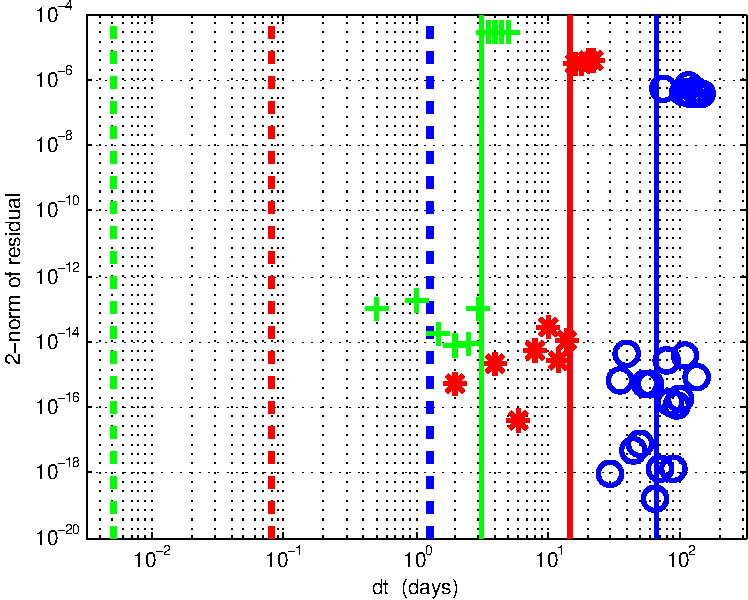
\includegraphics[width=3.5in,keepaspectratio=true]{figs/criticalconverge}
\caption{For grids with $\Delta x=2000$ m (blue), $\Delta x=500$ m (red), and $\Delta x=125$ m (green), respectively, we observe that the Newton solver for the nonlinear equations for a single time step converges up to a reasonably well-defined critical duration (solid line).  For $\Delta t$ smaller than the critical duration the Newton solver converges and the residual 2-norm is small ($10^{-19}$--$10^{-12}$).  Solid vertical lines are drawn according to a formula $\Delta t = C \Delta x^{1.1} / \max D$, a speculative but representative formula.  Dashed vertical lines are at $\Delta t_{expl}=\Delta x^2/\max D$, which would be much smaller timesteps.}
\label{fig:criticalconverge}
\end{figure}


\section{Results}

FIXME


\section{Discussion}

FIXME


\section{Conclusion}

FIXME


\small
\bibliography{ice_bib}  % generally requires link to pism/doc/ice_bib.bib
\bibliographystyle{agu}
\normalsize


\appendix

\section{An alternative with evolving hydraulic conductivity}  \label{app:evolveK}  If we use $P=p_i(W/W_{crit})^\sigma$, with nonevolving capacity $W_{crit}$, then we do not use \eqref{eq:capacityevolution}.  We can allow opening and closing of the drainage system by evolution of the hydraulic conductivity $K$, however.  Essentially this is proposed by \citet{Hewitt2011}, who has formula ``$\mathbf{q} = (k_0/\eta_w) h^3 (\mathbf{\psi} + \nabla N)$ and it is $h^3$, which is outside of $\nabla$ in this expression for flux, which evolves by physical opening and closing.

First let us suppose we have bounds on $K$, say $K_{min} \le K \le K_{max}$.  SUch bounds are in the literature \citep{FlowersClarke2002_theory}, and they can be enforced numerically by variational inequalities.  Now, as a example evolution model for $K$, one which is not even slightly-justified by physical opening and closing processes but which is used here for illustration, we choose
\begin{equation}\label{eq:evolvingK}
\frac{\partial K}{\partial t} = \alpha (2 K_{max} - K) \left(\left(\frac{W}{W_{crit}}\right)^2 - 1\right)
\end{equation}
where $\alpha\ge 0$ is constant and $K_{max}$ is constant.    The factor ``$(2K_{max}-K)$'' is introduced to have the right side depend in some way on $K$; this factor is always positive because of the bounds on $K$.  More significantly, if $W<W_{crit}$ then the drainage system is not full and the right hand side is negative, so there is ``closure'' in that sense, while if $W>W_{crit}$ then the right hand side is positive and the drainage system ``opens''.  It is very important, if we use an evolution equation for $K$, to look for alternatives to \eqref{eq:evolvingK} which have a \emph{physical} opening and closing process explanation.

Now we combine equations \eqref{eq:conserve}, \eqref{eq:flux}, \eqref{eq:potential}, \eqref{eq:shallowoverburden}, \eqref{eq:melthewitt}, and \eqref{eq:evolvingK}.  The result is fairly simple
\begin{align}
\frac{\partial W}{\partial t} &= \frac{\rho_i}{\rho_w( W_{crit})^\sigma} \nabla \cdot \Big(K W \nabla (H W^\sigma)\Big) + \frac{\rho_i^2 g}{\rho_w^2 L (W_{crit})^{2\sigma}} K W \Big|\nabla (H W^\sigma)\Big|^2, \label{eq:WKsystem} \\
\frac{\partial K}{\partial t} &= \alpha (2 K_{max} - K) \left(\left(\frac{W}{W_{crit}}\right)^2 - 1\right). \notag
\end{align}
This system is solved in PETSc code \texttt{petsc/kw.c}.  Apparently the solutions are just as stable as those for the $(W,Y)$ system in the main text, if not more so.


\section{Delayed connection of hydrology to basal resistance}  \label{app:delayedpw}  It is reasonable to suppose that the combined hydrology and ice dynamics system will cause an additional complication in creating a numerically-stable implementation, namely stiffness in the differential equations sense \citep{AscherPetzold}.  To a significant degree this possibility must be examined by numerical experiments.  The hydrology model itself will be implemented implicitly (section \ref{sec:implementation}), but it is the short timescales of that subsystem that might cause stiffness of the combined system, and for now we cannot allow these short hydrology timescales to force the entire model to be implicit, which is impractical.

Recall that this ``stiffness'' is the difference between the long time scales for interesting ice dynamical changes and the shortest time scales of the combined system.  For ice dynamics on the relevant grids the intrinsic time scale is closer to years or months than to days or minutes.  For the hydrology system, however, \citet{FlowersClarke2002_theory} say that ``the dynamics time step'' is ``seconds to minutes.''  Our consideration of similarity time scale for the Barenblatt solution in section \ref{sec:verif} is even more pessimistic, with $t_0\sim 10^{-4}$ s for the injection of a cubic kilometer of water.  The rest of PISM has admittedly-undesirable explicit time steps of a year or two to a few weeks, for ice flow mass continuity, with decreasing time step for higher spatial resolution.  High resolution ice sheet simulations would become impossible if such timesteps were forced to be hours or minutes or less.

In textbooks the word ''stiffness'' is used to describe a difficulty in solving ODE systems numerically.  As a standard textbook example, if you solve the ODE system
   $$\begin{pmatrix}\dot x \\ \dot y\end{pmatrix}
=  \begin{pmatrix} -100 & 99 \\ 99 & -100\end{pmatrix} 
\begin{pmatrix}x \\ y\end{pmatrix},$$
for $x(t),y(t)$ then you get a combination of exponential curves with time-scales
separated by a factor of about $200$.  Specifically,
   $$x(t) = c_1 e^{-t} + c_2 e^{-199t}.$$
Explicit time-stepping methods for this ODE system will fail if they do not take very short time steps to resolve the fast decay of the $e^{-199t}$ mode, but implicit method can recover a reasonably accurate solution to the slower $e^{-t}$ mode even if they use time steps much longer than that \citep{AscherPetzold}.  That fast mode is frequently uninteresting in the sense that it is does not describe the behavior of the system component we would like to measure.  For example, in the above ODE system we might want to compute $x(t)$ for large times, at which $e^{-199t}$ is undetectable, because we want to connect $c_1$ or the larger eigenvalue ($\lambda_1=-1$ for $e^{-t}$) to observations.

So we propose a modification to avoid stiffness, namely to lag (delay) the water pressure $P$ which enters into the calculation of yield stress $\tau_c$.  It is this last calculation, equation \eqref{eq:mohr-coulomb}, which couples to the ice dynamics; without this coupling fast hydrology timescales do not influence ice dynamics.

Our proposed delay is both a regularization to avoid stiffness and potentially a model for actual delay in the processes by which the basal resistance over large areas (i.e.~the area of one grid cell) evolves in response to changing water amount and pressure.

In fact, ice flow speed-up events at the start of the melting season are related to a delayed response of the drainage system \cite{Schoofmeltsupply, vandeWal2008}.  Part of this delay is modeled by equation \eqref{eq:capacityevolution}, where the hydrologic capacity evolves in response to changes in water amount and (instantaneous) pressure.  But the period over which the lagged water pressure below is computed, a additional, pre-determined exponential time $\tau$ (equation \eqref{eq:tauaverage} below), can be regarded as a contributor to the response time of the system's plastic till morphology to fluctuations in subglacial water.

We introduce an additional lagged variable $\hpw$ which approaches $P$ with a characteristic time scale $\tau>0$,
\begin{equation}
\label{eq:pwslow}
  \frac{\partial \hpw}{\partial t} = -\frac{1}{\tau} (\hpw - P).
\end{equation}
Parameter might $\tau$ have value of weeks or months, because it should compare to the time steps of the ice dynamics calculation.  Equation \eqref{eq:pwslow} itself should be solved implicitly, coupled to the other state variables $W,Y$ of the hydrology model.

Solutions $\hpw(t,x,y)$ approach $P(t,x,y)$ exponentially, with characteristic time $\tau$. Recall that the solution of the simple homogeneous differential equation $dy/dt = - (1/\tau) y$ is $y(t) = y_0 \exp\left(-(t-t_0)/\tau\right)$ for the initial condition $y(t_0)=y_0$.  On the other hand, solving \eqref{eq:pwslow} represents an averaging of values of $P$ so as to compute $\hpw$.  In fact, solutions $\hpw(t)$ of \eqref{eq:pwslow} can be written
\begin{equation}\label{eq:tauaverage}
\hpw(t) = \hpw(t_0) e^{-(t-t_0)/\tau} + \frac{1}{\tau} \int_{t_0}^t e^{-(t-s)/\tau} P(s)\,ds.
\end{equation}
The integral on the right side is a weighted average of the influence of $P(t)$.  More weight is given in this integral to those $s$-values which are within $\tau$ of $t$ than for earlier $s$-values.  In practice we add differential equation \eqref{eq:pwslow} to the coupled PDE system formed by equations \eqref{eq:nonlineardiffusion} and \eqref{eq:coupledcap}, and we solve these differential equations together by implicit timesteps, so integral equation \eqref{eq:tauaverage} only shows the manner in which $\hpw$ is a delayed version of $P$.

If this delayed-water-pressure model is used then we compute yield stress by
\begin{equation} \label{eq:mohr-coulomb-delayed}
  \tau_c = c_0 + (\tan{\phi}) (p_i - \min\{p_i,\hpw\})
\end{equation}
instead of \eqref{eq:mohr-coulomb}.  Thereby the ice dynamics model only ``sees'' the delayed/averaged water pressure $\hpw$.


\section{Computation of Jacobian} \label{app:jacobian}  FIXME: OUT OF DATE

Order all $N$ values $W_{i,j}$, over the whole grid, into an $N$-vector $\bW$.  Recall the equations which define ODEs $dW_{i,j}/dt = F_{i,j}(\bW)$.  To compute the Jacobian we find derivatives of the right side functions $F_{i,j}$ with respect to the unknowns $W_{k,l}$.  The Jacobian matrix $J(\bW)$ is an $N\times N$ matrix where $N$ may be $10^4$ or $10^8$, but there are only a few nonzero entries per row, as shown in Figure \ref{fig:sparsity}. 

For simplicity define $C_x =\gamma/\Delta x^2$, $C_y = \gamma/\Delta y^2$.  The diagonal entries of $J(\bW)$ are these:
\begin{align} \label{eq:jacdiag}
\frac{\partial F_{i,j}}{\partial W_{i,j}} &= \frac{C_x}{2} \Big[(W_{i+1,j}^\sigma - 2 W_{i,j}^\sigma + W_{i-1,j}^\sigma) - \sigma  W_{i,j}^{\sigma-1} (W_{i+1,j} + 2 W_{i,j} + W_{i-1,j})\Big] \\
   &\qquad + \frac{C_y}{2} \Big[(W_{i,j+1}^\sigma - 2 W_{i,j}^\sigma + W_{i,j-1}^\sigma) - \sigma  W_{i,j}^{\sigma-1} (W_{i,j+1} + 2 W_{i,j} + W_{i,j+1})\Big]. \notag 
\end{align}
The other four entries are in off-diagonal positions.  To describe them, also define $G(a,b) = (\sigma+1) a^ \sigma/2 + b (\sigma a^{\sigma-1} - b^{\sigma-1})/2$.  Then
\begin{align} \label{eq:jacoffdiag}
\frac{\partial F_{i,j}}{\partial W_{i+1,j}} &= C_x\, G(W_{i+1,j},W_{i,j}), &\qquad
\frac{\partial F_{i,j}}{\partial W_{i-1,j}} &= C_x\, G(W_{i-1,j},W_{i,j}), \\
\frac{\partial F_{i,j}}{\partial W_{i,j+1}} &= C_y\, G(W_{i,j+1},W_{i,j}), &\qquad
\frac{\partial F_{i,j}}{\partial W_{i,j-1}} &= C_y\, G(W_{i,j-1},W_{i,j}). \notag
\end{align}

\begin{figure}[t]
\centering
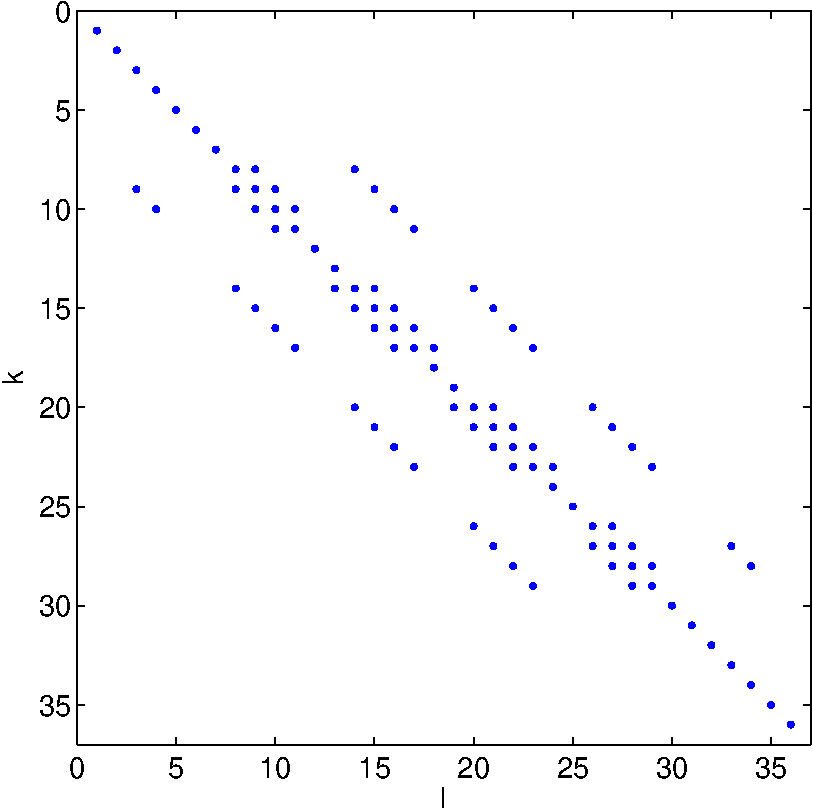
\includegraphics[width=2.5in,keepaspectratio=true]{figs/sparsity.pdf}
\caption{Sparsity pattern of Jacobian matrix, from a small grid with $N=36$ points.}
\label{fig:sparsity}
\end{figure}


\section{Prototype codes with descriptions} \label{app:prototypes}

\begin{itemize}
\item \texttt{matlab/baren.m}: \quad This Matlab/Octave simply displays snapshots of the Barenblatt solution as a movie.
\item \texttt{petsc/matlabprint.h}: \quad Small collection of C language routines which puts PETSc DMDA-based Vec objects in Matlab/Octave ascii files.
\item \texttt{petsc/context.h}: \quad C language routines which set default constants and compute the Barenblatt exact solution.
\item \texttt{petsc/porous.c}: \quad Runs a time-stepping simulation of the verification case, a vertically-integrated porous medium equation, using an implicit finite difference method implemented in C.  Uses PETSc TS (time-stepping) object.  The TS object attaches a SNES object to do Newton method solutions of the equations for each implicit time steps.  Has a subroutine to compute the right-hand-side $F_{ij}$ of the spatially semi-discretized equation for $W$, and one to compute the Jacobian $J=[\partial F_{i,j}/\partial W_{k,l}]$.  Requires PETSc 3.2.
\item \texttt{petsc/bh.c}: \quad Runs a time-stepping solution of \eqref{eq:Weqnfd} and \eqref{eq:Yeqnfd} for the $(W,Y)$ state space model.  Initial condition is a Barenblatt state for $W$ and $Y=Y_0$.
\item \texttt{petsc/kw.c}: \quad Runs a time-stepping solution of equations in a $(W,K)$ state space model.  Contrived, nonphysical evolution of $K$, namely by equation \eqref{eq:evolvingK}.  Initial condition is a Barenblatt state for $W$ and $K=K_0$.
\end{itemize}

\end{document}
